\documentclass[12pt]{article}
\usepackage[parfill]{parskip}
%Mathematical TeX packages from the AMS
\usepackage{amssymb,amsmath,amsthm} 
%geometry (sets margin) 
\usepackage[margin=1.25in]{geometry}
\usepackage{enumerate}
\usepackage{graphicx}
\usepackage{amsfonts}
\usepackage{hyperref}

\theoremstyle{plain}% default
\newtheorem{thm}{Theorem}[section]
\newtheorem{lem}[thm]{Lemma}
\newtheorem{prop}[thm]{Proposition}

\theoremstyle{definition}
\newtheorem{defn}{Definition}[section]
\newtheorem{conj}{Conjecture}[section]
\newtheorem{exmp}{Example}[section]

\theoremstyle{remark}
\newtheorem*{rem}{Remark}
\newtheorem*{note}{Note}
\newtheorem{case}{Case}

\begingroup
    \makeatletter
    \@for\theoremstyle:=definition,remark,plain\do{%
        \expandafter\g@addto@macro\csname th@\theoremstyle\endcsname{%
            \addtolength\thm@preskip\parskip
            }%
        }
\endgroup
%=============================================================
%Fancy-header package to modify header/page numbering 
%
\usepackage{fancyhdr}
\pagestyle{fancy}
\lhead{Wesley Chen, Brandon Sim}
\chead{} 
\rhead{\thepage} 
\lfoot{\small Applied Math 120} 
\cfoot{} 
\rfoot{\footnotesize Automating Brain Tumor Detection in MRI Images} 
\renewcommand{\headrulewidth}{.3pt} 
\renewcommand{\footrulewidth}{.3pt}
\setlength\voffset{-0.25in}
\setlength\textheight{648pt}

%=============================================================

\begin{document}

\title{Automating Brain Tumor Detection in MRI Images}
\author{Wesley Chen, Brandon Sim}

\maketitle
\tableofcontents
\newpage

\section{Introduction and Motivation}
% this is a comment
% introduction, motivation, previous work here

\section{Methodology}
\subsection{Watershed Segmentation}

\subsection{Symmetry Analysis}

\subsection{Symmetry Analysis, Centroid Analysis}

\section{Results}

\section{Discussion and Future Work}


\section{Conclusion}
In conclusion, we...(talk about what we did, general overview stuff that we said in the presentation - how we combined two methods, one more traditional method, one more specific to our application, etc, etc)

We invite you to view all the code at \url{https://github.com/bksim/images}.
\section{References}
\begin{enumerate}
\item MATLAB bla bla
\item
\end{enumerate}

\section{Appendix A: Watershed Segmentation Images}
% how to include graphics (put all images in same folder)
\begin{figure}[!h]
	\centering
		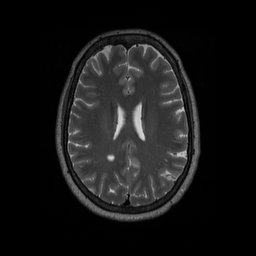
\includegraphics{original.jpg}
	\caption{Slice 79, Axial.}
\end{figure}

\section{Appendix B: Symmetry Analysis Images}


\section{Appendix C: MATLAB code}
\subsection{Watershed Segmentation Code}
Description of what file does.
\subsubsection{filename.m}
\begin{verbatim}
code here
\end{verbatim}

\subsection{Symmetry Analysis Code}
Description of what file does.
\subsubsection{filename.m}
\begin{verbatim}
code here
\end{verbatim}

\subsection{Anomaly Detection Code}
Description of what file does.
\subsubsection{filename.m}
\begin{verbatim}
code here
\end{verbatim}

\subsection{Miscellaneous Code}
Description of what code does (python file will go here)
\subsubsection{python.py}
\begin{verbatim}
code here
\end{verbatim}
\end{document}